\documentclass{article}%
\usepackage[T1]{fontenc}%
\usepackage[utf8]{inputenc}%
\usepackage{lmodern}%
\usepackage{textcomp}%
\usepackage{lastpage}%
\usepackage{authblk}%
\usepackage{graphicx}%
%
\title{Expression and Differentiation between OCT4A and Its Pseudogenes in Human ESCs and Differentiated Adult Somatic Cells}%
\author{Tiffany Cooley}%
\affil{Institute of Bioinformatics and Biosignal Transduction, College of Bioscience and Biotechnology, National Cheng{-}Kung University, Tainan, Taiwan}%
\date{01{-}01{-}2013}%
%
\begin{document}%
\normalsize%
\maketitle%
\section{Abstract}%
\label{sec:Abstract}%
SAN DIEGO {-} Two Tiam1 cells became infected with a type of liver cancer, and other cancers spreading through the body while delivering the cancer drug duchennevirin, researchers reported Tuesday in the journal Cancer Epidemiology, Biomarkers \& Prevention.\newline%
A data monitoring system was installed at the St. Luke's Healthcare System's San Diego Memorial Hospital to detect the tumor, the researchers said.\newline%
These results suggest that toxic "trigger cell" patients {-}{-} a population more typically associated with types of cancer such as melanoma {-}{-} are at risk.\newline%
"We thought there would be a distinct low rate of these trigger cells," said co{-}author James Pericard of the St. Luke's Health System. "But that changed dramatically."\newline%
A trigger cell {-}{-} a white cell that is expressed with certain genes such as melanoma receptor {-}{-} passes on many tumors in the body to another cell that can survive and metastasize. The trigger cell appears in about half of treated cancer patients and the other half is not.\newline%
It produces several genes on tumor skin surfaces called "acids" that trigger inflammation in the surrounding tissue. These inflammatory acids are believed to trigger tumors to grow more rapidly, and sometimes spread to other tissue.\newline%
Tiam1 cells that had mutated into the trigger cells emerged in tumors found in 32 patients with chronic kidney disease, 29 patients with primary lung cancer and only 15 patients with sarcoma.\newline%
There were no differences in cancer outcomes for the trigger cells in the patients with sarcoma and those with chronic kidney disease and primary lung cancer, the researchers reported.\newline%
Sulcomastoma is a cancer of the lymphatic vessels that feed the liver. Sarcoma is a cancer of the soft tissue in the bone marrow.\newline%
Each patient had different tumors with different types of liver cell types. The encouraging results did not come from patients with liver cirrhosis, which may be caused by transplants.\newline%
Chronic kidney disease was not associated with the trigger cells, and those that are, they found in the liver were linked to rare but significant liver dysfunction.\newline%
The study is not designed to show whether risk factors for liver disease in the trigger cells are the cause of the liver cancer, said Dr. Stephen Hart of Brown University, who was not involved in the research.

%
\subsection{Image Analysis}%
\label{subsec:ImageAnalysis}%


\begin{figure}[h!]%
\centering%
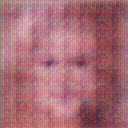
\includegraphics[width=150px]{500_fake_images/samples_5_393.png}%
\caption{A Close Up Of A Person Wearing A Suit And Tie}%
\end{figure}

%
\end{document}